% !TEX root = main.tex
\chapter{Introduzione}
Nel progetto sono stati affrontati alcuni dei vari problemi che riguardano l'intelligenza artificiale. In questa relazione spiegheremo quali soluzioni sono state adottate, i vantaggi e gli svantaggi e alcuni miglioramenti che possono esser fatti al nostro progetto

\section{Strategie}
Per svolgere il progetto di IA-LAB sono state implementate 4 strategie in maniera incrementale:
\begin{itemize}
  \item FIFO WAIT: la strategia usa la politica fifo come politica di scelta degli ordini. 
  \item FIFO: Simile alla precendente, ma in caso di ostacolo che non permette di servire un ordine, l'ordine viene messo al fondo.
  \item LOW PENALITY: strategia che si basa sulla penalità per effettuare la scelta dell'ordine.
  \item HARD: a differenza delle altre 3 strategia, questa permette di gestire più ordini in contemporanea. Come la precedente si basa sulle penalità.
\end{itemize}

Ogni strategia è stata suddivisa in fasi dove ogni fase si occupa di uno specifico sotto-problema. Questa suddivisione ci ha permesso sia uno sviluppo incrementale all'interno della stessa strategia, sia tra strategie diverse, dove è bastato andare a sviluppare in modo più articolato una fase oppure nell'inserire nuove fasi.

\subsection{Astar}
Tutte le strategia utilizzano il modulo Astar per pianificare dei piani che permettano al nostro robot di spostarsi da un punto A a un punto B. Il punto A è la posizione del robot al momento della pianificazione mentre il goal (il punto B) è dato dalla cella destinazione. La cella destinazione può essere un dispenser, un cestino o un tavolo. Il modulo astar calcolerà quali sono i 4 punti di accesso alla nostra destinazione e si fermerà non appena arriverà a uno di esso.

Il modulo A* può terminare fornendo un piano, oppure può fallire. Per memorizzare il piano creato vengono usate due strutture:

\begin{lstlisting}
(deftemplate plane 
	(slot plane-id) 
	(multislot pos-start) 
	(multislot pos-end) 
	(slot direction) 
	(slot cost) 
	(slot status (allowed-values ok failure))
)
\end{lstlisting}
\begin{lstlisting}
(deftemplate step-plane 
	(slot plane-id)
	(slot action)
	(slot direction)
	(multislot pos-start)
	(slot father)
	(slot child)
)
\end{lstlisting}

La struttura step-plane indica i vari passi per eseguire il piano plane. I piani vengono memorizzati in modo tale che il robot non debba ripianificare più volte uno stesso percorso. Vengono memorizzati solo i piani principali; nel caso in cui un piano fallisca il piano "riparatore" non viene memorizzato.

\chapter{Strategie}
\section{Strategia FIFO WAIT}
La prima strategia che illuestreremo è la FIFO WAIT. \'E una strategia molto semplice, dove il primo ordine che arriva è l'ordine che viene servito. Vi sono vari casi per completare un ordine:\begin{itemize}
  \item Ordine Accepted: un ordine di questo tipo verrà completato solo quando verranno consegnate al tavolo tutte le consumazioni richieste.
  \item Ordine Delayed: un ordine di questo tipo verrà completato solo quando verranno consegnate al tavolo tutte le consumazioni richieste. Rispetto al caso precedente le consumazioni non potranno esser consengate fin quando il tavolo non verrà pulito e le consumazioni buttate nel cestino.
  \item Ordine Finish: un ordine di questo tipo verrà completato solo quanto verrà pulito il tavolo e il robot butterà lo sporco nei vari cestini.
\end{itemize}

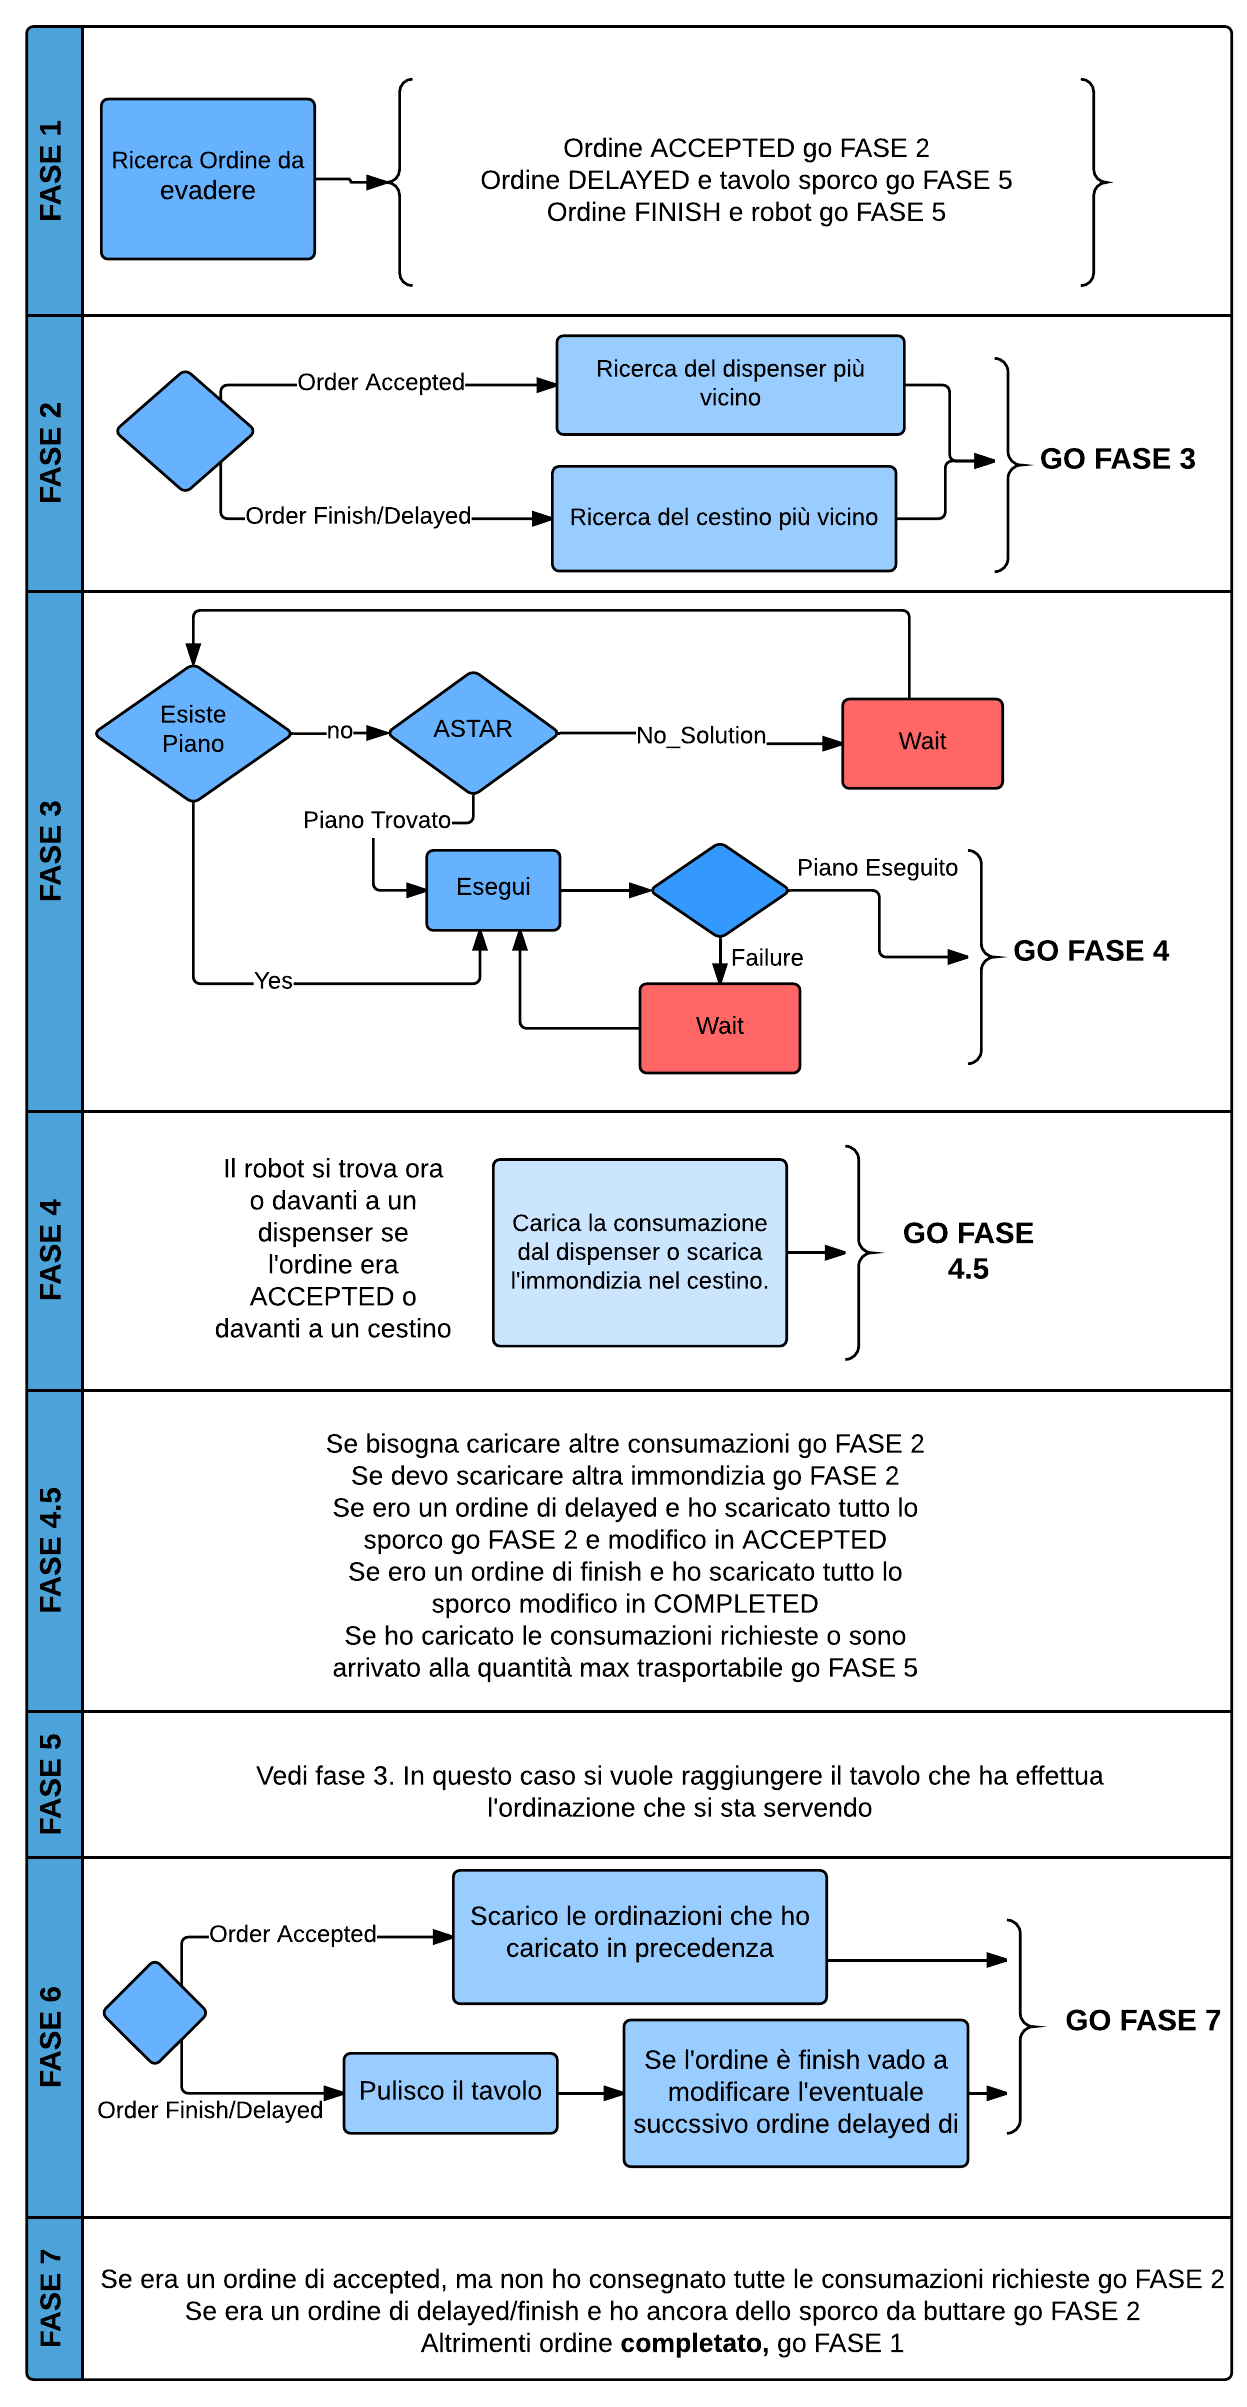
\includegraphics[width=\textwidth]{schema-fifo-wait.png}

Come possiamo vedere dallo schema abbiamo suddiviso la nostre strategia in 7 fasi:
\begin{itemize}
  \item Fase 1: Nella prima fase viene individuato quale sarà l'ordine da servire. 
  \item Fase 2: In questa fase si andrà ad individuare quale sarà il cestino o il dispenser presso il quale il nostro robot dovrà recarsi. La ricerca del cestino o del dispenser dipene dal tipo di ordine.
  \item Fase 3: In questa fase il robot arriverà alla destinazione prefissata. Per far ciò deve prima calcolare un piano con A* e poi eseguirlo. Il piano viene calcolato solo se non ne esiste già uno. In caso A* non trovi soluzione il robot esegue una wait e prova a ricalcolare A* fin quando non trova una soluzione.
  Quando il robot ha un piano per raggiungere la sua destinazione lo esegue. Nel caso in cui il piano fallisca il robot esegue una wait e prova a rieseguirlo.
  \item Fase 4: Il robot a seconda dell'ordine che sta servendo si troverà davanti un dispenser per caricare delle consumazioni (ordine accepted) oppure davanti a un cestino per buttare lo sporco (ordine delayed o finish).
  \item Fase 4.5: Questa è fase di controllo in cui il robot decide a seconda dell'ordine cosa deve fare. Per esempio se era un ordine accepted e ha caricato solo i 'food' e gli mancano i 'drink' dovrà ritornare alla fase 2; analogamente se era un ordine di finish o delayed e deve ancora buttare dello sporco.
  \item Fase 5: Identica alla fase 3 tranne per il fatto che la destinazione sarà un tavolo.
  \item Fase 6: Il robot in questa fase si trova in una posizione in cui può operare sul tavolo. Nel caso di ordine accepted rilascio tuttle le consumazioni caricate; in caso di ordine finish o delayed pulisco il tavolo.
  \item Fase 7: In questa fase controllo se l'ordine può essere considerato completato.
\end{itemize}

\subsection{Vantaggi e Svantaggi}
Vantaggio di questa strategia è sicuramente la semplicità e l'intuibilità con la quale il sistema funziona. L'idea di questa strategia, oltra alla politica di evasione degli ordini che può essere cambiata in qualsiasi momento andando solo a modificare la fase 1, è quella che il mondo è dinamico e lo è con una certa frequenza. L'assunzione dalla quale siamo partiti è che le persone si spostano e si spostano molto frequentemente. Da questo risulta evidente che se per arrivare in una determinata posizione incontro un ostacolo (una persona) la mossa più conveniente è quella di aspettare.
Se prendiamo in considerazione le teorie di Rodney Brooks in cui afferma che un comportamento intelligente è attribuibile da un osservatore esterno che vede l'agente interagire con l'ambiente, allora in alcune circostanze il nostro agente potrebbe non dimostrare tale comportamento intelligente. Se una persona rimane, anche se per pochi step in una posizione lungo il percorso dell'agente, il nostro agente invece di aggirarla e dimostrare un comportamento intelligente continuerà a provare a muoversi lungo la sua direzione fin quando la persona non si sarà spostata. Questo comportamento porta anche a situazioni di deadlock. Essendo in un ambiente simulato anche le persone non hanno un comportamento intelligente, supponendo che una persona si vuole spostare in direzione sud e il robot in direzione nord si arriva in una situazione di stallo. Per ovviare a questa problematica abbiamo implementato la strategia FIFO.

\chapter{Strategie}
\section{Strategia FIFO}